\documentclass[]{../resources/final_report}
\usepackage{graphicx}
\usepackage[hidelinks]{hyperref}
\usepackage{amsmath}
\usepackage{amssymb}
\usepackage[toc,page]{appendix}
\usepackage{wrapfig}
\graphicspath{{../resources/images/}}

\newcommand{\Reals}{\mathbb{R}}


%%%%%%%%%%%%%%%%%%%%%%
%%% Input project details
\def\studentname{Roger Milroy}
\def\reportyear{2019}
\def\projecttitle{Autonomous Micro Air Vehicles: Enhanced Navigation in GPS denied environments.}
\def\supervisorname{Professor Sara Bernadini}
\def\degree{BSc (Hons) in Computer Science (Artificial Intelligence)}
\def\fullOrHalfUnit{Full Unit} % indicate if you are doing the project as a Full Unit or Half Unit
\def\finalOrInterim{Interim Report} % indicate if this document is your Final Report or Interim Report

\begin{document}

\maketitle

%%%%%%%%%%%%%%%%%%%%%%
%%% Declaration

\chapter*{Declaration}

This report has been prepared on the basis of my own work. Where other published and unpublished source materials have been used, these have been acknowledged.

\vskip3em

Word Count: 6028

\vskip3em

Student Name: \studentname

\vskip3em

Date of Submission: December 6th 2019

\vskip3em

Signature: Roger Milroy

\newpage

%%%%%%%%%%%%%%%%%%%%%%
%%% Table of Contents
\tableofcontents\pdfbookmark[0]{Table of Contents}{toc}\newpage

%%%%%%%%%%%%%%%%%%%%%%
%%% Your Abstract here

\begin{abstract}

All robotic systems that are mobile require an understanding of their position in order to 
maneuver effectively, avoid obstacles and carry out useful tasks.
In the context of Micro Air Vehicles (MAVs) the situation is more challenging due to the 
twin problems of noisy sensors and limited computation. There are many different approches to 
solving this problem and most if not all of them use the Kalman Filter in order to fuse sensor 
data and provide optimal estimates of state.

%% Objectives
The main objective of this project is to implement the newly proposed technique of 
Hybrid Inference (HI) as an improvement on the Kalman Filter in the context of position 
estimation in MAVs in a simulated environment. The secondary aim is to demonstrate it on the 
DJI Matrice 100 with the Jetson Nano as the onboard computation platform.

The project is based upon a technique of Monocular Simultaneous Localization and Mapping (SLAM) 
which also recovers absolute scale. This integrates visual data and absolute measurments, such 
as Inertial Measurment Unit (IMU) data. It uses an Extended Kalman Filter to integrate the sensor 
data which is what this project will be replacing and evaluating the impact. My initial assessment 
of the Monocular SLAM technique was that the technique was useful but implemented on a specific 
platform, the Parrot AR drone. Upon further investigation I discovered that the implementation
was mostly platform agnostic. This led me to prioritise HI over reimplementing the Monocular SLAM 
technique.

%% Software Engineering approach
The first terms work has not provided much opportunity for applying Software Engineering principles
due to the bulk of the work being that of mastering new theory, learning new technologies and 
assembling existing projects. I was however able to apply them to the design of the architecture of the system as a whole and 
in the HI demonstrator.

%% Background Theory
Monocular SLAM with scale recovery is the technique upon which hybrid inference will be demonstrated. 
Kalman filters are the existing solution and also form the basis of the hybrid inference solution,
as it uses the same problem formulation. HI is the general technique that fuses existing 
mathematical techniques with neural networks. The report explores both theoretical and technical 
aspects of all these techniques.

%% Work Completed
The report details a summary of the work that has been completed this term. Learning how to
use ROS and Gazebo, setting up the TUM ardrone and hector packages that I am building upon. 
And finally, implementing a demonstrator of the HI technique on a synthetic dataset. 

%% Second term work.
Some additional challenges have been identified during the course of this work. First is that HI as described 
in the paper, deals with a simplified linear dynamic model that does not have inputs to the system.
The dynamic model that describes MAVs must include external inputs for control. Reformulating the 
graphical model to account for this is the first new challenge that I had not identifiend in the 
initial project plan. The second challenge is temporal. With a Kalman Filter, it is possible to 
estimate future states and the uncertainty of those postulated states. This is critical for dealing 
with latency issues in the real time control environment that MAVs present. The current formulation 
of the underlying graphical model does not allow for future reasoning, solving this is necessary to
enable HI to be used this domain.

Finally I describe the work to be completed in the second term. The provided Gantt chart shows the
projected timeline.

\end{abstract}
\newpage

%%%%%%%%%%%%%%%%%%%%%%
%%% Introduction
\chapter{Introduction}


%%%%%%%%%%%%%%%%%%%%%%
%%% 
\section{Motivation}

Micro Air Vehicles (MAVs) popularly known as quadcopters, have become ubiquitous in recent years 
with prices dropping across a range of sizes of drones. This has lead to their deployment across 
a number of sectors and applications. These include videography, where most of us will have seen 
their output, all the way to assessing and counting endangered species with numerous other 
applications in between.

One major challenge is that of fixing position accurately. Most solutions use some kind of 
satellite navigation solution to fix absolute position. This is effective in outdoor environments
but ineffective in a number of environments, such as anywhere indoors, in forests or underwater.
In these environments it is necessary to rely on inertial sensors as well as image or other data. 
These are fused in an Extended Kalman Filter to produce a single estimate of position.
The main issue with these techniques is that absent regular fixes of known positions, estimates of
position accumulate error.

If we can reduce the rate that this error accumulates, this opens up the space of viable environments
that automated systems can operate in and increases their usefulness.


%%%%%%%%%%%%%%%%%%%
%%% Objectives
\section{Objectives and Contributions}

\subsection{Objectives}
The main objective is to apply the newly proposed technique of Hybrid Inference (HI)
\cite{Satorras2019CombiningGA} to the problem of position estimation in MAVs. HI integrates 
existing mathematical models with Neural Networks in order to improve inference performance in 
both low and high data regimes.

In addition I aim to demonstrate HI using onboard computation, taking position estimates that 
come from inertial sensors and visual SLAM systems. I will use a Jetson Nano for computation, 
mounted to a DJI Matrice 100 quadcopter.

For the first term, the key objectives were to validate the technique by implementing it on a 
small synthetic dataset, to demonstrate in Gazebo the Monocular SLAM with scale recovery technique 
\cite{Engel:Camera-basedNav} upon which the Hybrid Inference will be implemented and finally to 
validate the Jetson Nano platform for computation. All these objectives were successfully achieved.

The objectives for the second term are to implement Hybrid Inference for state estimation completely 
and demonstrate it on a simulated quadcopter in Gazebo. Secondary goals are to integrate the 
Jetson Nano onto the Matrice 100 and adapt the code to work with the DJI OSDK. Finally to demostrate 
the fully realised project in precision figure flying in order to compare with the results of 
Engel et al. \cite{Engel:FigureFlying}.

% \subsection{Contributions}
% To apply this technique to a new problem instance and to evaluate whether it improves on current 
% state estimation techniques. To suggest its viability for onboard deployment on resource constrained
% platforms.

% TODO does this need to be an entire chapter or is a section more appropriate
% if so where should it go?
\chapter{Professional Issues}
% TODO change if staying as a chapter.
\section{Professional Issues}
% write about how a particular issue has been of concert to you in the project.

% core ethical concern in this project is that of application.

The core ethical concern for me during this project is that of application.
The application of technology is where the bulk of the societal impacts occur. 
But for the people developing these technologies there are two somewhat distinct situations. 
There is the case where we develop a particular application, like Facebook which has a particular
direct impact on the world which we can then evaluate as to whether it is beneficial or not. 
Then there is the case where we develop a technology that underlies applications and maybe 
enables new features or improves the efficacy of existing features, we could also think of 
these as tools used for creating other applications. This situation is harder to evaluate as 
to whether the technology is beneficial or not. 
A good example of this is the Internet, as a technology it is neutral but it has enabled many 
applications that people would see as mostly good such as improving access to learning for 
hundreds of millions of people. At the same time it has enabled criminals to perpetrate new 
forms of crime such as blackmailing people over intimate photos they have gained access to 
illegally. It is not clear how to weigh the relative merits of the applications so it is also
hard to evaluate the technology itself. One of the core challenges of this situation is whether 
there is a responsibility to mitigate the risk of negative uses of the technology.

I would consider my project to fall into the second category. This is because the primary goal 
of this project is to demonstrate a technique that can reduce errors in pose estimation. This 
could enable more precise positioning of drones for longer periods of time, which could open up 
some environments that currently are more challenging for drones to operate in. The main examples
are indoors, in forests or anywhere where GPS coverage is intermittent, including cities with a 
large number of skyscrapers in close proximity, and finally underwater.
Thus it is an enabling technology rather than an application of existing technology.

-- Positive applications REDO...
I want to explore some of the potential applications of my project, both what I would consider 
to be beneficial and those I would consider undesirable. 
On the positive end of the spectrum are applications like automated search and rescue. By reducing
dependence on GPS signals, in the best case drones could be deployed fully autonomously to locate
missing persons in a variety of domains where they cannot currently and if done with large numbers 
of drones it could drastically reduce the time taken to find missing persons.
Another positive application could be in increasing reliability and accuracy for consumer navigation 
applications. This could improve the customer experience by reducing the amount of erroneous 
instructions given by these applications.
It is also possible that by improving localisation accuracy indoors that a wider range of indoor 
robotics applications could be enabled. This is towards the bottom because there are a wide array 
of other challenges that must be overcome and navigation accuracy is not the greatest of them.


-- Negative applications
There are in contrast a number of potentially harmful applications. These are mostly concerned with 
the enabling of more autonomous weapons. Currently there are many consumer drones deployed with some 
measure of autonomous capability such as Return-to-Home capabilities. We have not yet seen any military 
use of autonomous MAVs however improved precision of flight may open up this area. A small thought 
experiment we could carry out would be to think about the incident at Gatwick in December 2019 where 
around 1000 flights were disrupted \cite{Gatwick_Airport} and considering how that would have been 
different if the drones involved were autonomous. And again if there were multiple, it would be extremely 
difficult for the authorities to effectively prevent interference with airport operations. To extend 
the thought experiment, imagine that the drones were fitted with explosives. This is not too much of 
a stretch given other events such as those in Venezuela in August 2018 \cite{Caracas_drone} where that was exactly 
the assertion.

Looking at military capabilities and plans, it is very likely that swarming drones will be put into 
service in the not too distant future. This is due to two primary factors. One is cost. The unit cost of 
military hardware in the UK increases at a high rate with unit costs for RAF aircraft increasing at 11.5\% \cite{RUSI_defence_costs}. 
This means that the numbers of vehicles, ships and aircraft has been falling. Drones have the potential to reverse this trend by 
equipping large expensive human operated vehicles, ships and aircraft with large numbers of cheaper, 
smaller drones. There has been much talk of swarming drones to overwhelm conventional defences and this 
is one expression of the interest the military has in autonomous drones.

At the same time the technologies enabling the autonomous operation of drones also lowers the barriers 
that prevent smaller but malicious actors from using them to cause harm. In fact ISIS and other terrorist 
organisations have already been known to use remotely operated drones to carry out attacks \cite{something}. 
It is not that big of a step for them to deploy them autonomously. In many cases the tools are there to 
program a predefined flight path.

What is not so clear is to what extent improving navigation accuracy enables autonomous operation. 
It is a core competence of an autonomous device \cite{rttas} but not the only one. And depending on the 
environment and desired accuracy it can be considered a solved problem. If operating outdoors and 
needing accuracy of around 1m, GPS navigation is sufficient. It is only in more complex terrain and 
with higher accuracy requirements that you may struggle. In my opinion there are other more important 
enabling factors, the most important of which are the tools that support the development of autonomous 
behaviour and simplify that process.

In conclusion, I think that there are risks of negative outcomes given this technology however I don’t 
think that it enables any greater risks than already exist and at the same time I don’t think it increases 
the likelihood of any other risks appreciably.

A lot depends on the efficacy, and efficiency of the solution. In all likelihood it is unlikely to be 
much more effective than the EKF and is more computationally expensive than is feasible for small scale 
applications. This limits the risk considerably.





%%%%%%%%%%%%%%%%%%%%%%
%%% Planning and Timescale
\chapter{First Term Planning}

\section{Original Plan}

The original plan delayed the bulk of the implementation until the second term. While this was 
not unreasonable given the learning curve for each of the technologies involved, if I stuck to 
the original plan I would have been faced with a huge amount of work with little to base it on.
There was also quite a lot of uncertainty about the state of the TUM codebase. The original 
assumption was that the code had been written specifically to work with the Parrot AR drone as 
it was the platform on which they demonstrated \cite{Engel:Camera-basedNav}.
This would have meant rewriting the code to work in ROS and be platform independent. When I found 
that was not the case it changed the dynamics of the project quite significantly and led to the 
new plan.

I have included below the original plan Gantt Charts that detail milestones and timescales.
\\
% Gantt chart?
\begin{figure}[h]
  \centering
  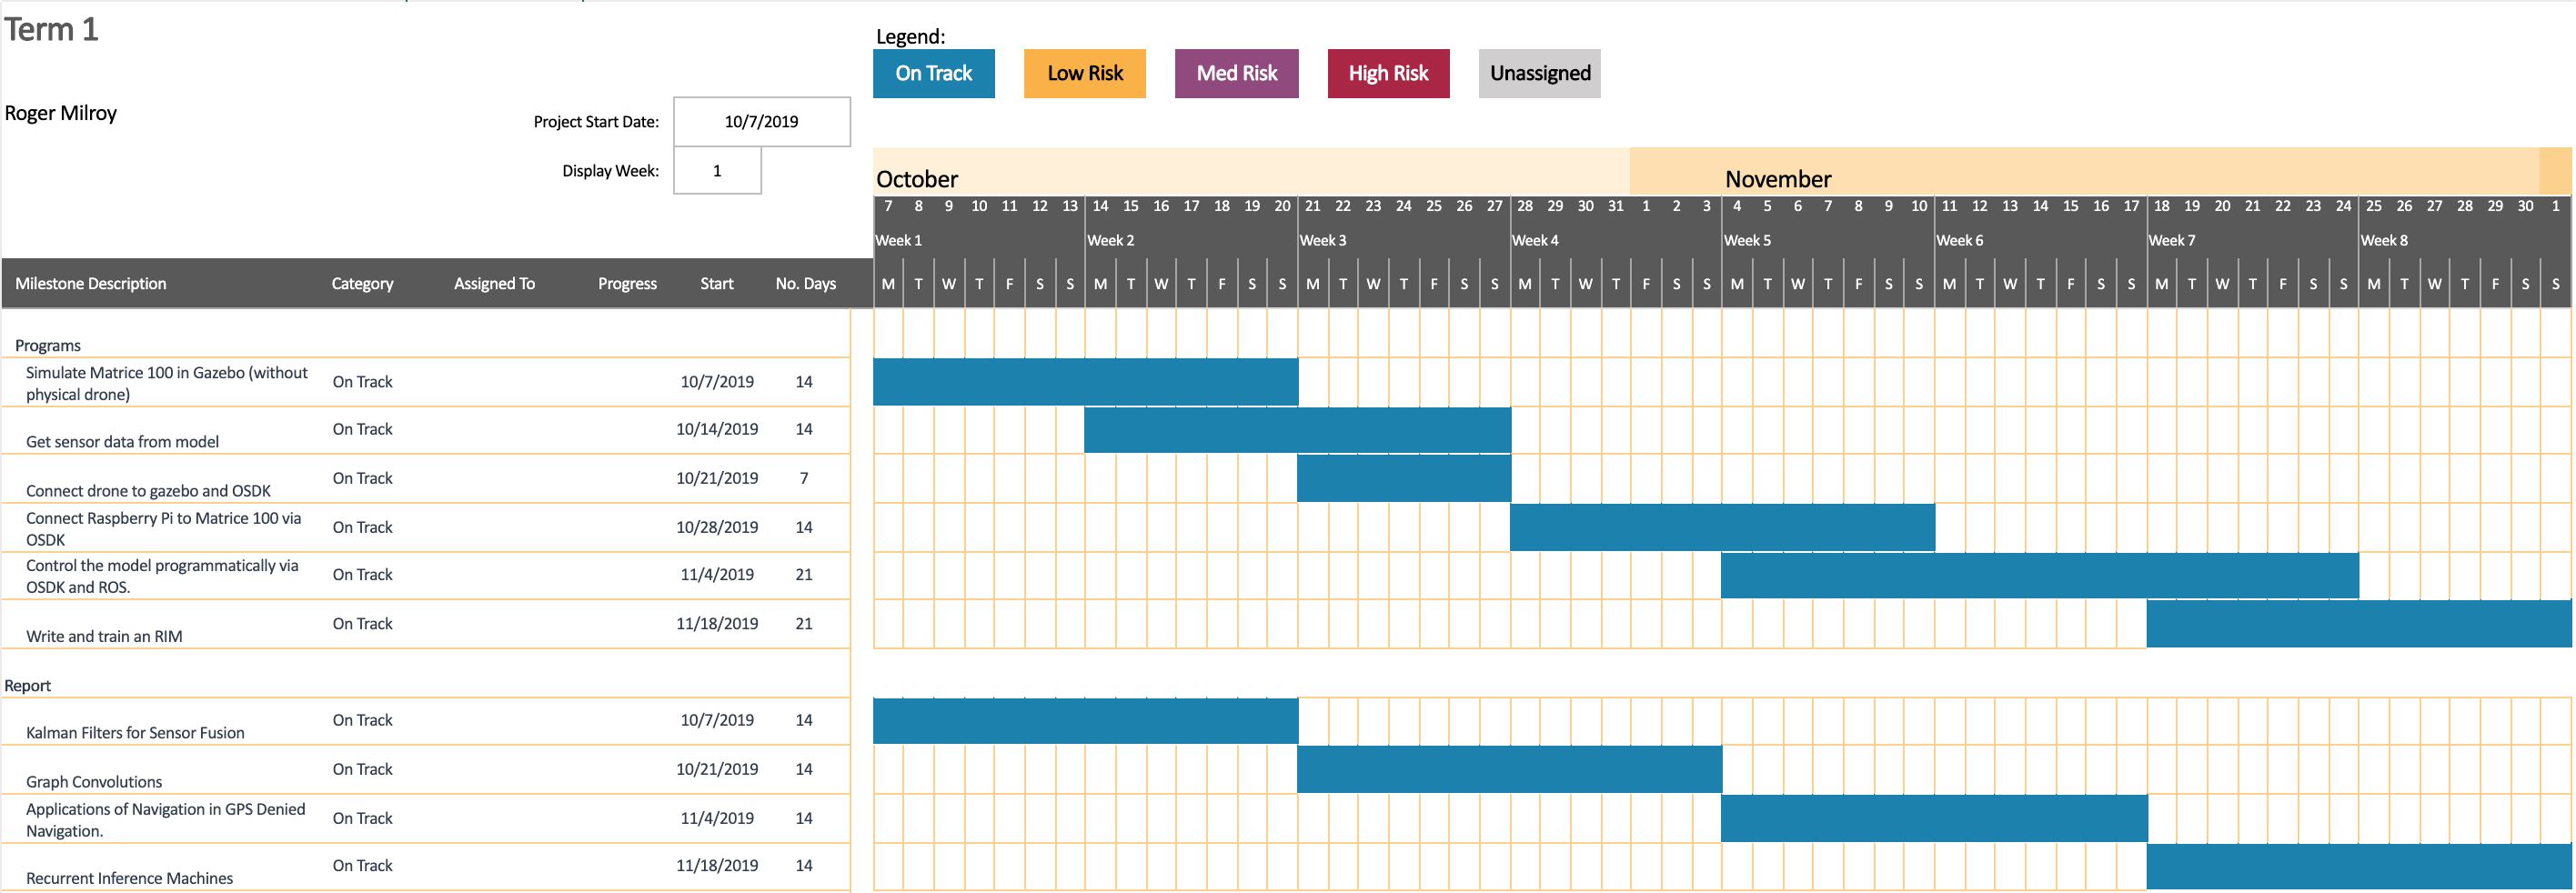
\includegraphics[width=\textwidth]{Term1Ganttv1.png}
  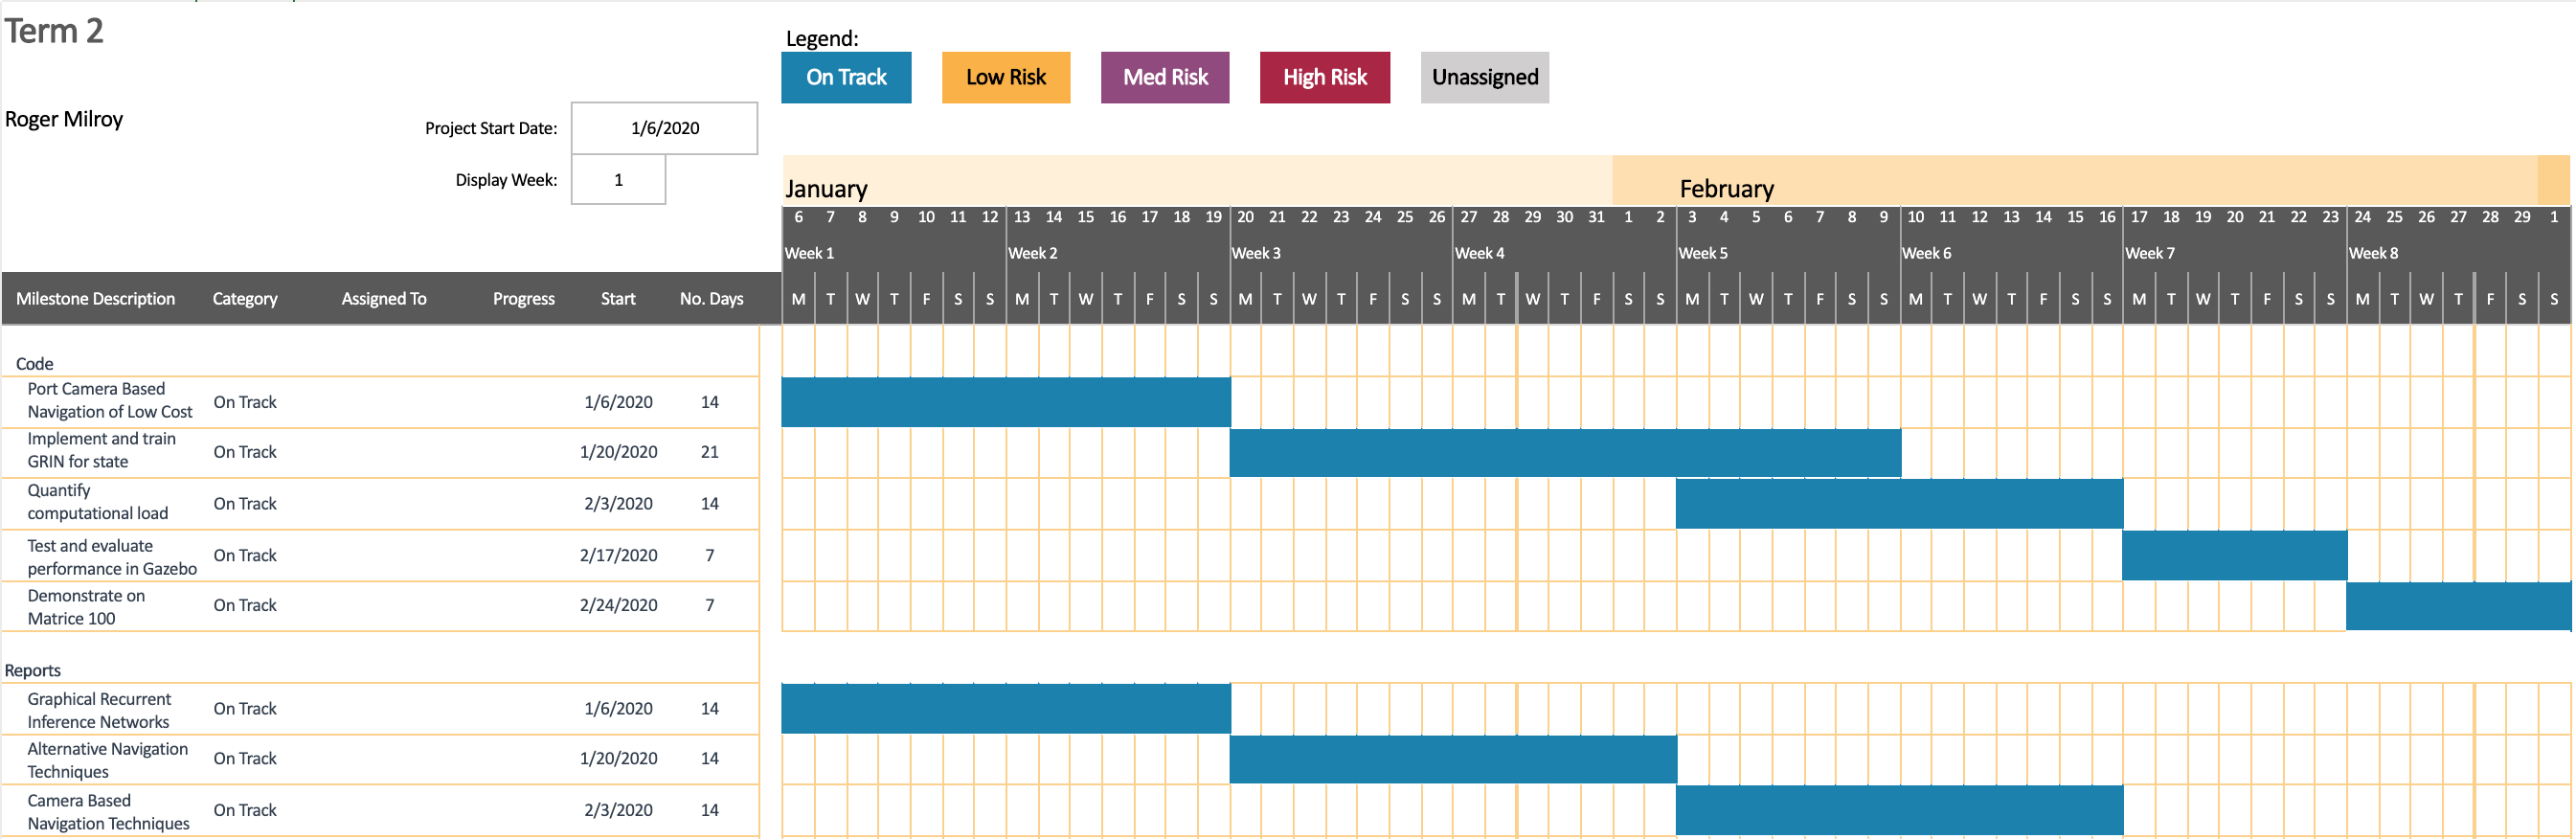
\includegraphics[width=\textwidth]{Term2Ganttv1.png}
  \caption{Original Plan Gantt Charts}
  \label{}
\end{figure}



\section{Revised Plan}

While working on the project the outlook changed quite significantly when I found the code for 
the Monocular SLAM with scale recovery was open source. This meant that I could directly build 
upon their work and extend it instead of spending the bulk of the project reimplementing their 
technique. This enabled me to pivot to focusing more on the implementation of HI. 
Under the new plan most of the first term is spent getting simulation working with the existing 
code base. I also implement a simple version of the HI technique on synthetic 
position data.

I replanned and the following are the updated milestones and associated dates. I will elaborate 
on the work to be done in the second term at the end of the report.
\\
\begin{figure}[h]
  \centering
  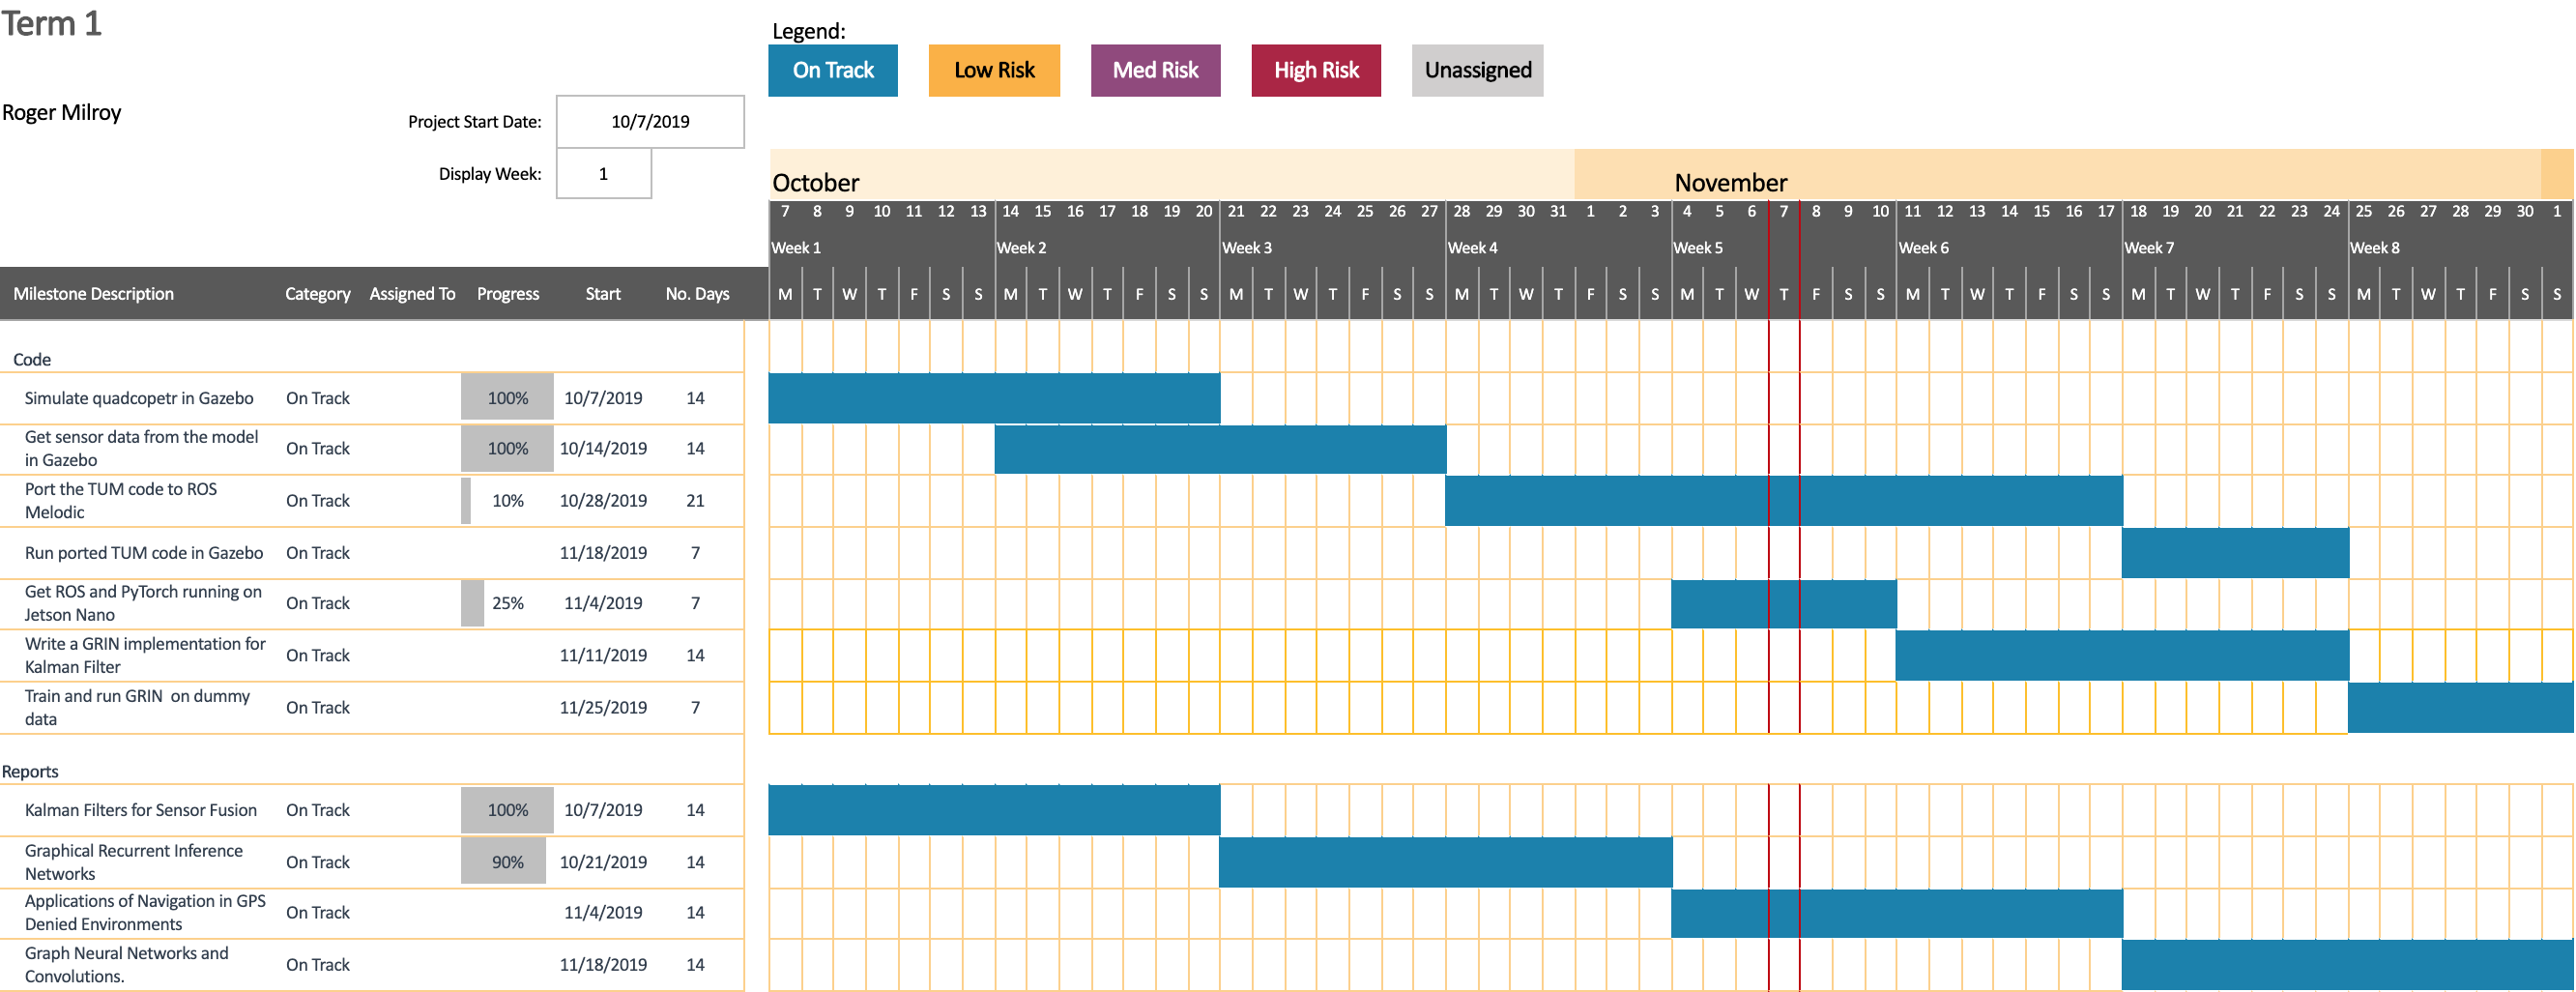
\includegraphics[width=\textwidth]{Term1GanttChart.png}
  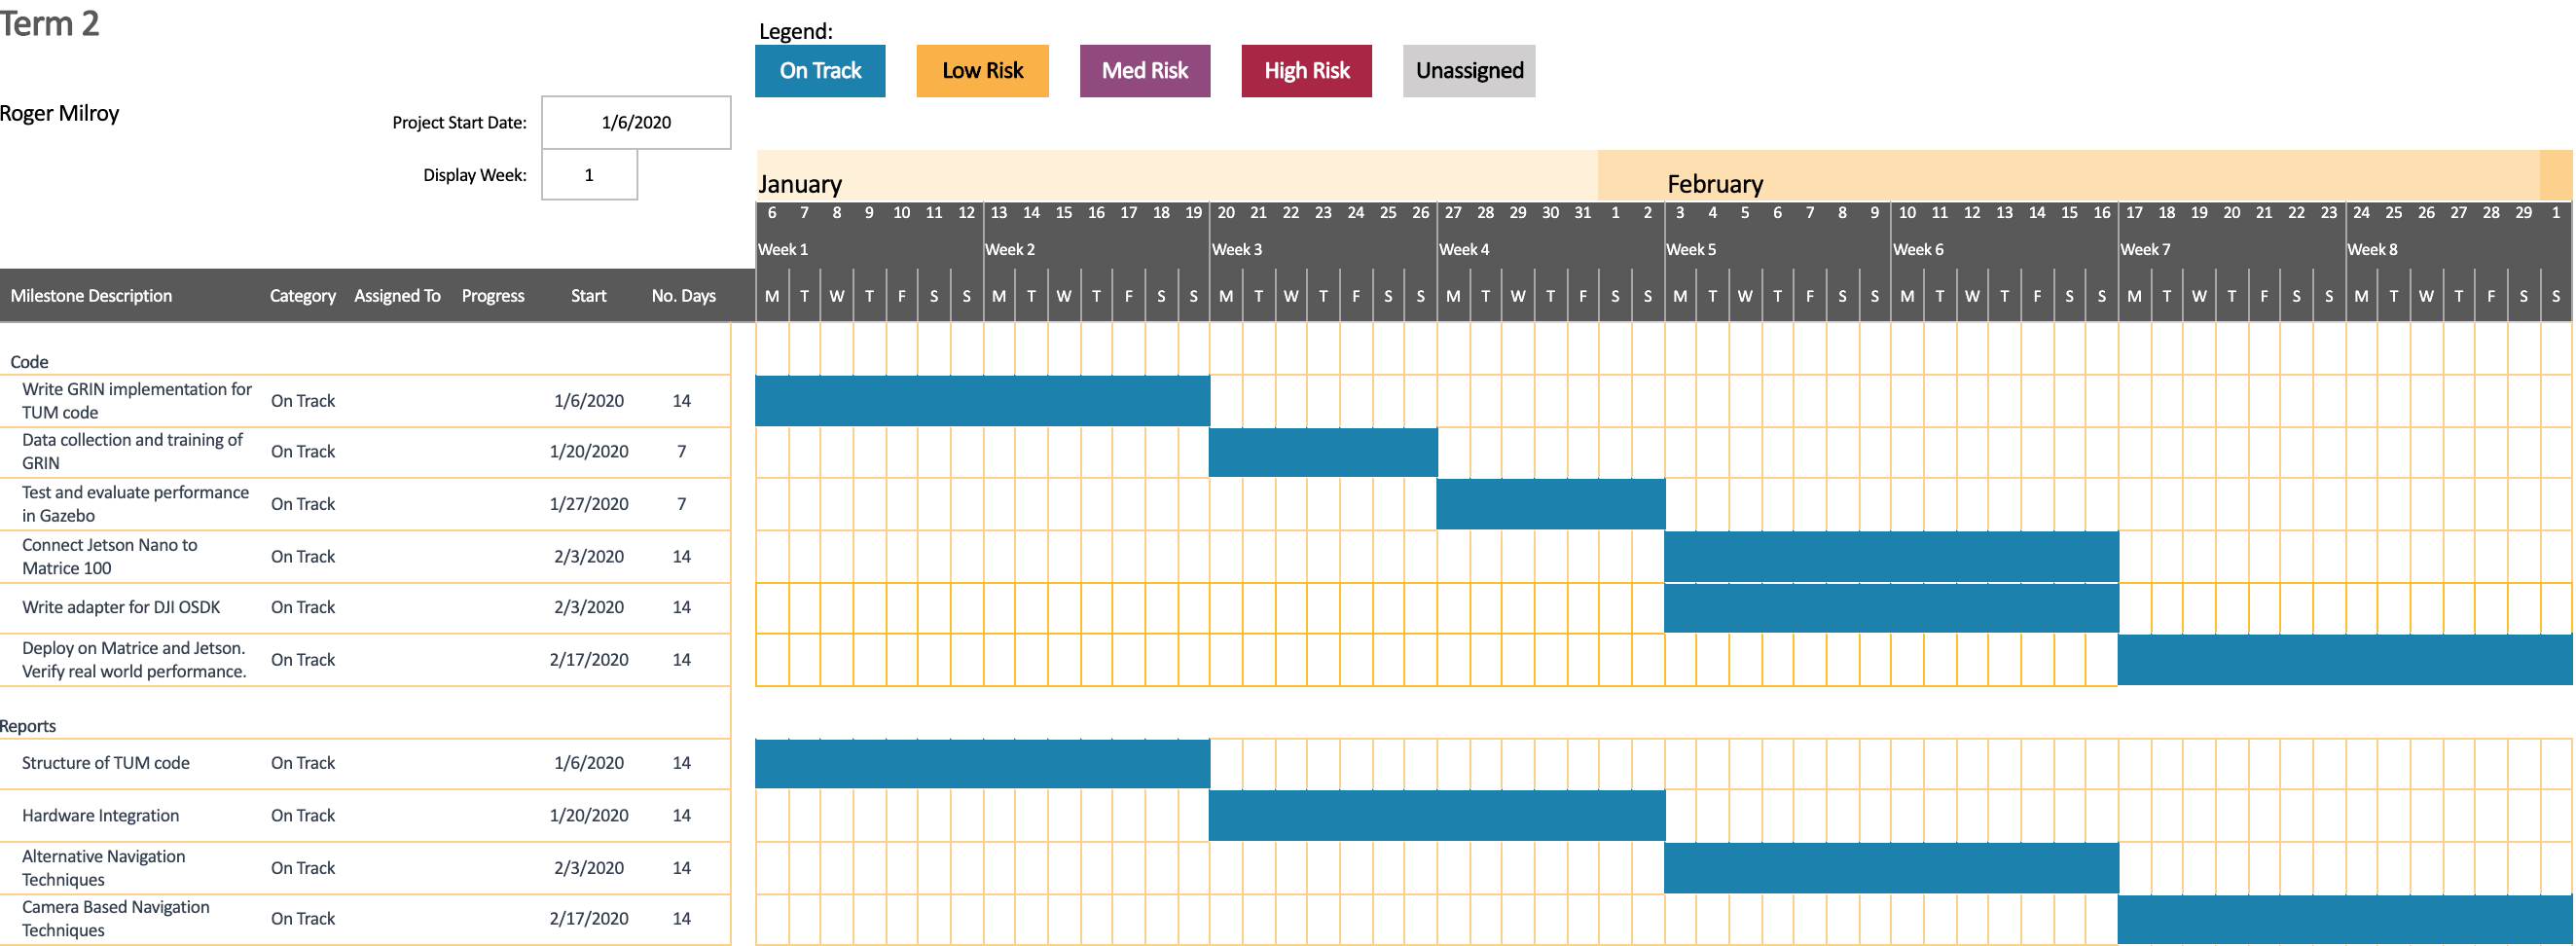
\includegraphics[width=\textwidth]{Term2GanttChart.png}
  \caption{Revised Plan Gantt Chart}
  \label{}
\end{figure}


%%% Software Engineering
\chapter{Software Engineering}

\section{Tools}

\subsection{Version Control System}
I used git as my version control system, and GitHub as my remote. I actually have a number of 
repositories because for the ROS section of the project it was necessary to modify existing 
projects code. I created a private fork of the relevant projects and then modified them as necessary.

I have separate branches for development, reports and for each feature that I am working on. 
These last ones are only temporary and are closed as soon as the feature is tested and integrated 
back into development. The workflow that I have decided upon is to use development for completed 
features once they have been tested. This does not imply that development is stable however so I 
only release code considered stable to master. The idea is that master should only contain stable 
code and be safe to use at any point.

\subsection{Project Task Tracking}
I used Trello in order to organise and keep track of tasks while completing them. I use a single 
board with To Do, Doing and Done lists. Each task is a card and has an associated due date.
This is really useful to stay on track and quickly assess the state of the project at a glance. 
I also used this while replanning as I could evaluate each task and see whether it was still 
relevant in the new context. One additional advantage of using Trello is that it keeps track of 
history and has space for lists within tasks allowing them to be broken up into sub tasks.


\subsection{Development Tools}

I used both VSCode and PyCharm as Development Environments. They both have different advantages 
and disadvantages and I used VSCode for the C++ work and PyCharm for the Python work.
For ROS development I have an Ubuntu VM with the relevant dependencies installed as well as the 
two IDEs I just mentioned.

I used the built in testing framework for Python, 'unittest' for testing. This provides a very 
similar framework to JUnit and allows for clear easy test setup and management.


\section{Development}

\subsection{Design}
% ROS
ROS lends itself to modular code however the packages that I am working with and building on have 
very mixed engineering approaches. To date my work has been composing the projects and getting them 
to run so Software Engineering practices have been limited to thinking about the design of the full 
implementation.

Unfortunately ROS is not particularly conducive to Test Driven Development (TDD) as there is no 
framework that enables testing outside of nodes. I can test the components of each node in the 
standard fashion, which I plan to do though this will apply more next term.

All of the design decisions that I have taken, both for implementations this term and the plans 
for future work, have been in the pursuit of modularity.

It is widely accepted that good code should be modular and reusable where possible. There are 
aspects where this is obviously not possible, such as configurations and any implementation 
specific work, but this should where possible be isolated and offer abstract interfaces.

With respect to the packages I have chosen, the hector stack and the TUM work, they have to some 
extent taken this approach but only really within the project. 
This complicates my work somewhat but at the same time using these as the base allows me to explore
 more advanced concepts over reimplementing the functionality of these modules.
I will be writing adapters to enable the existing codebase to interact.

For the proof of concept of Hybrid Inference, the Dataset and the Linear Motion Model that creates 
synthetic data I implemented them as separate classes. A standard Object Oriented approach and used
composition where necessary.


\subsection{Testing Strategy}

Due to the limitations that I have regarding support for testing frameworks, particularly in ROS, 
I have relied a lot on sanity checking at each stage while testing formally as many sections as 
possible. Integration tests are particularly important for my project as I have a variety of 
different technologies that need to work together across a number of interfaces.
This will become important in the next stage of the project as that is when the different components 
start to interact and when I will be looking to start deploying code onto the hardware.

To this point I have thoroughly Unit Tested the proof of concept of HI, the 
Dataset and Linear Motion model.


\subsection{UML}
%% UML
I have included the package diagram that describes the high level design 
of the project as well as the class diagram of the HI demonstrator.

\begin{figure}[h]
  \centering
  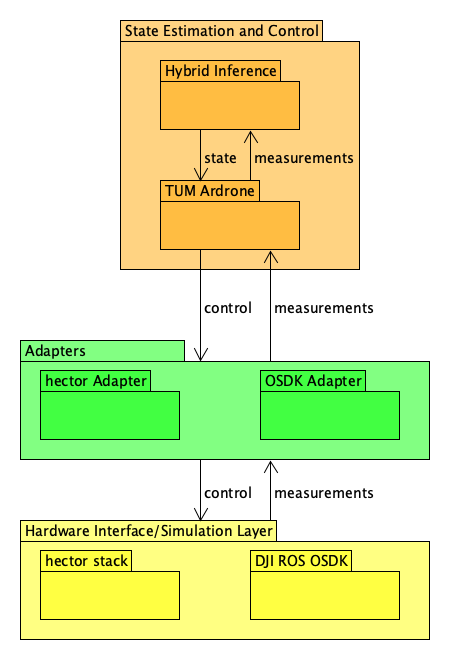
\includegraphics[height=0.30\textheight]{hybrid-inference-package-uml.png}  
  \caption{Package diagram of the project.}
  \label{}
\end{figure}


\begin{figure}[h]
  \centering
  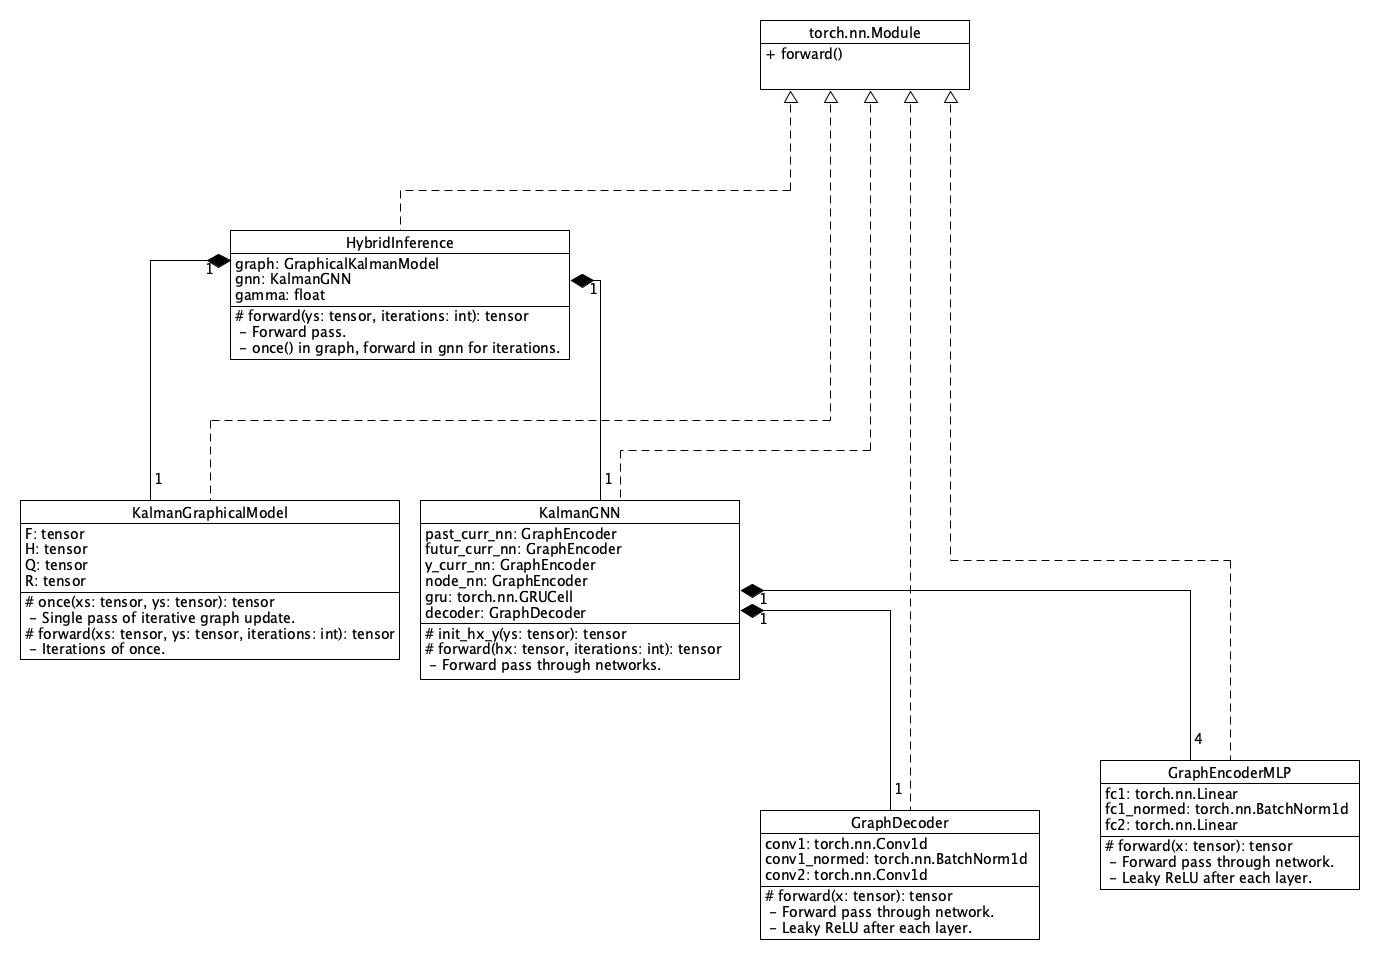
\includegraphics[height=0.36\textheight]{hybrid-inference-uml.png}
  \caption{Class diagram for Hybrid Inference}
  \label{}
\end{figure}


%%%%%%%%%%%%%%%%%%%%%%
%%% Literature Review
\chapter{Background Theory}
% This is where the background theory will go too.

\section{Literature Survey}

%% some stuff about what to read for what.

\section{Gazebo and ROS}

%% Explainer on Gazebo and ROS and see if there are references for them.
In order to demostrate the effectiveness of the code that I have written it is essential that it is 
demonstrated first in a simulated environment. This neccesitates using Gazebo as it is the industry 
standard robot simulation software. In a similar token the industry standard robot development 
framework is ROS, which works with Gazebo and so this is the primary technology stack that I am 
using.

Both ROS and Gazebo are very powerful but they don't have a particularly easy onboarding process. 
For learning basic ROS concepts I used a service called Robot Ignite Academy that has some simple 
tutorials to make the process of learning the ROS way of doing things a bit quicker. One challenge I 
had at the very early stage was understanding what ROS actually was. There are very few high level 
descriptions of it, and they are certainly not the first topic on the ROS tutorials pages.

What I learned was that ROS is a paradigm of programming robots as well as an 
implementation of that paradigm. The paradigm is that each peice of code on the robot is a Node 
that takes data from a Topic, processes it and outputs data for other Nodes to use on a Topic. 
Some Nodes don't do both of these and some also directly effect change in the robot, think of a 
Node that controls a motor, it would read and change the voltage to the motor.

The other concepts that make up ROS are that of Services which are synchronous and Activities that 
are asynchronous, both operate on the Client - Server pattern. Topics as I mentioned are 
communication channels that operate on the Publisher-Subscriber pattern. And Messages which actually 
have quite a bit of intricacy and can be quite confusing. There are 3 types of Message. Regular 
Messages that are published to Topics. Then Actions and Services also define their own formats of 
messages. They will often use standard messages defined for use in Topics but additional message 
formats will be generated for each Action or Service.
%% Need to add references

\section{Monocular SLAM with scale recovery.}

%% put a UML diagram of the library layout/dependancies.
In two related papers \cite{Engel:FigureFlying}\cite{Engel:Camera-basedNav}, Engel et al. present a 
technique of Monocular SLAM that is able to recover absolute scale. In order to understand why 
this is significant and important some background is needed.

The primary problem of visual SLAM techniques is that of creating a high quality depth map of the 
surroundings. This can be accomplished by stereo vision, which is where two cameras are used and the 
distance and rotation between the two of them are known. Ideally the axes are aligned and there is 
no rotation between the cameras though this can vary depending on the specific requirements.
This can be extended to use three or more cameras but in the more general case, known as structure 
from motion, it is possible to use a single camera. In that case we are trying to recover the 
transformation and rotation between frames. This is possible however it is not possible to recover 
absolute scale from this technique as we don't know the absolute distances between frames. In the 
stereo case the information about the position and orientation of the cameras relative to each other
is known a priori and so we can recover absolute scale.

Engel et al. tackle the issue of scale recovery by using data from the IMU which usually consists of 
3 accelerometers and 3 gyroscopes and often a magnetometer or other absolute scale sensors such as 
altimeter or barometer. This is standard equipment on quadcopters as it is needed to maintain stability. 
They use the information provided by this sensor in conjunction with the structure from motion 
equations in order to recover the absolute scale. In order to estimate the scale factor which is 
usually referred to as $\lambda$ they take a maximum likelihood approach, which in simple terms 
means they estimate the $\lambda$ that maximises the likelihood of the $x$ and $y$ positions 
measured by onboard sensors. In order to solve successfully they turn it into the negative log 
likelihood which you then minimize. This is a common trick and in this case it leads to a closed 
form solution for $\lambda$. This is important as it reduces the computational cost and makes it 
more feasible with onboard computation. In the paper they use a Parrot AR drone which has very 
constrained payload and computation capacity so they use offboard computation.

In the second paper \cite{Engel:FigureFlying} they present the full system including the scale 
estimation and demonstrate its effectiveness in position flying and holding.


\section{State Estimation}

%% Kalman Filters
The core method used for state estimation in the face of noisy sensors is the Kalman Filter. It is 
used by Engel et al.\cite{Engel:Camera-basedNav} for state estimation and sensor fusion which are 
its most common uses in this field.

Let us formally define the problem. The system we are measuring is assumed to be characterised by a 
Hidden Markov Model, this is how Kalman characterised the dynamical system we are interested in \cite{Kalman1960ANA}. 
In this formulation there are hidden states $x$ and observations $y$. The system being a Hidden 
Markov Process means that it is characterised by the following equations:

\begin{align}
  x_t &= Ax_{t-1} + Q_t \\
  y_t &= Hx_t + R_t
\end{align}

Where $A$ is the transition matrix from time $t-1$ to $t$, and $\xi_t$ is the noise at time $t$. 
This represents that the model dynamics are stationary so $A$ is fixed but there is noise in 
transitions, that is transitioning between states is non-deterministic. $H$ is the measurement 
matrix and $R_t$ is the noise in the measurements. This models the reality of noisy measurements 
that may not be correct and in fact represents the true problem. We want to recover the true 
measurements despite being given noisy observations.

The Kalman Filter gives an optimum estimate of $x$ which I will call $x^*$ by deriving three matrices 
$\Phi^*$, $P^*$ and $\Delta^*$:

\begin{align}
  \Delta^*(t) &= A_{t+1;t}P^*_tH^T_t[H_tP^*_tH^T_t]^{-1} \\
  \Phi^*_{t+1;t} &= A_{t+1;t} - \Delta^*_{t+1;t}H{t} \\
  P^*_{t+1} &= \Phi^*_{t+1;t}P^*_tA^T_{t+1;t} + Q{t}
\end{align}


Note that in the Kalman formulation he also considers non stationary dynamic systems. In our 
situation we assume stationarity which allows us to drop the time specification on the transition 
matrices $A$ and $H$.

With these matrices, the optimal estimate of state at time $t+1$, $\hat{x}_{t+1|t}$ is given by 

\begin{align}
  \hat{x}_{t+1|t} &= A^*\hat{x}_{t|t-1} + \Delta^*_ty_t
\end{align}

The estimation error $x'$ and covariance of the error, cov $x'$ are

\begin{align}
  x'_{t+1|t} &= A^*x'_{t|t-1} + Q_t \\
  \text{cov } x' &= P^*_t
\end{align}

From this we can see that the Kalman Filter is an iterative process where each iteration builds upon 
the previous best estimate of state. To recover the estimates of the true measurements we simply 
need to multiply the best estimates of the state by the measurement matris $H$.

Kalman and Bucy extended the Kalman filter that, in the form stated above works for discrete time, to the 
continuous case the year after the original paper \cite{Klmn1961NewRI}.

These equations only apply to linear dynamic models which is something of an issue given that most 
real life applications are of non linear dynamic systems. To solve this we use Taylor expansions to 
linearise our non-linear models around the current state \cite{ExtendedKalmanNasa}. This does 
unfortunately add a large overhead as we need to re linearise at each time step to avoid 
accumulating linearisation errors.

%% Graph Neural Networks
\section{Graph Neural Networks}

% Explain the premise behing GNNs
As the technique I am implementing makes use of Graph Neural Networks (GNNs) I will first explore
what GNNs in relation to regular neural networks (NNs).

\subsection{Neural Networks}
To understand GNNs it is first necessary to understand some key properties
of NNs. The first is that NNs are Universal Function Approximators \cite{Hornik}
That is given sufficient hidden layer neurons a neural network can approximate any real valued function 
no matter how complex. This is the basis for their power and flexibility.

This doesn't come without drawbacks however. The cost of this flexibility is that 
training a universal function approximator (or a feed forward network with an arbitrarily 
large hidden layer) is not necessarily feasible in computational terms or in terms of 
the amount of data required.

The paradigm of learning that NNs ascribe to is called representation learning. That is learning
meaningful representations of data in order to achieve some useful outcome.

In order to overcome this limitation there has been great progress in 
formulating specific architectures of neural networks. Some good examples of these 
are Convolutional Neural Networks (CNNs) and Residual Networks (ResNets). 
One of the keys to these models successes is that they constrain the neural architecture.
For these two in particular they constrain the model to Euclidean space and 
particular dimensions within this space. This restriction means that 
the resulting network is no longer a universal function approximator but that 
also reduces the amount that the network has to learn like about the rules of Euclidean space and what
a dimension within the data is. It is precisely these restrictions that 
enable such networks to learn with fewer data samples and to a greater accuracy
than would be possible otherwise.

This can be rephrased with a slightly different interpretation by seeing the constraints on
the network as introducing inductive biases into the model. This biases it to learn
certain features of the dataset and not others. 

\subsection{Graphs}

% Define Graphs?
We define graphs as a collection of nodes (also known as vertices though I will use the word node from now on) 
and a collection of edges over those nodes.
Graphs are prevalent across many different areas of science and are a particular focus of
many Computer Scientists. Famous examples of graph algorithms include Djistra's Algorithm, Depth First Search and A star.
Why are graphs so prevalent? Well the answer is that they have great expressive power to 
represent objects or concepts and their relations.

The flexibility of graphs is mirrored in the great variety of operations that we might want 
to carry out over them. At the same time there is a huge number of different configurations 
of graphs varying over degree of connectivity of each node, whether edges are weighted or directed, 
containing cycles or not and whether the graph changes at all.
Whether the edges represent different kinds of relation and what information each node contains.

\subsection{Graph Neural Networks}

We consider each node to have a vector label or feature. This may contain information about edges or not.
If we were to try and apply CNNs or RNNs to graphs in this form, we could do so by stacking the node 
features and operating over that. In this case the node features would contain the information about edges.

This is not ideal because it enforces or biases the model to a particular ordering of nodes where there 
might not be one. We could overcome this by computing over all possible orderings of nodes.
This would however add significant computation. \cite{graphoverview}
It also prevents the model from exploiting the graphs inherent structure, as it had been 
folded into the nodes themselves. It is clear then that this is not the best approach.

% GNN
\subsubsection{Original GNN}
Now I will explain the original GNN proposed by \cite{GNN}. The following explanation is drawn from \cite{graphoverview} with some rewording. 
The goal of the GNN is to learn an embedding $ \emph{h}_x \in \Reals_s $ of each node $x$ which contains the information 
from the node and its locality. This embedding is then used to generate an output $\emph{o}_x$ of each node, often called the decoding step,
where the embedding of each node generates a prediction of some kind for example the node labels.

In order to compute these embeddings and outputs we define two parametric functions, the first is $f$ a 
local transition function which is shared by all nodes, and $g$ the local output function. These are defined as:

\begin{align}
  \textbf{h}_v &= \emph{f }(\textbf{x}_v, \textbf{x}_{co[v]}, \textbf{h}_{ne[v]}, \textbf{x}_{ne[v]})\\
  \textbf{o}_v &= \emph{g }(\textbf{h}_v, \textbf{x}_v)
\end{align}

where $\textbf{x}_v$, $\textbf{x}_{co[v]}$, $\textbf{h}_{ne[v]}$, $\textbf{x}_{ne[v]}$ are the features of v, the features of its edges, 
the states, and the features of the nodes in the neighborhood of $v$, respectively.

This can be condensed by stacking vectors to form matrices. Then we have $\textbf{X}$, $\textbf{X}_N$, $\textbf{O}$ and $\textbf{H}$ 
consisting of all features, the features of the nodes, the outputs and the states respectively. In this form we then have global transition 
function $F$ and global output function $G$.

\begin{align}
  \textbf{H} &= F(\textbf{H}, \textbf{X})\\
  \textbf{O} &= G(\textbf{H}, \textbf{X}_N)\\
\end{align}

The GNN takes inspiration from Banach's fixed point theorem \cite{khamsi_kirk_2011} and uses the following iterative scheme to 
compute the states:

\begin{align}
  \textbf{H}^{t+1} = F(\textbf{H}^t, \textbf{X})
\end{align}

This converges to a stable $H$ exponentially fast for any start point of $\textbf{H}_0$

We use NNs for the parameterised functions $\emph{f}$ and $\emph{g}$.

As stated in \cite{GGNN} the model is trained using the Almeida-Pineda algorithm \cite{Almeida}\cite{Pineda} where 
the states are computed to convergence at which point the output and losses are computed. 
The gradients of the weights in the transition function and output fuction networks are computed from
this final state and the weights updated according to the optimisation algorithm selected.


% Adding Recurrence.
\subsubsection{Recurrence}

An extension or variation of the GNN is the Gated Graph Neural Network (GGNN). The key reason for the introduction
of the GGNN is to reduce the restrictions on the transition function. Rewording what was stated in \cite{GGNN} the 
paper that proposes the GGNN they outline the challenge of the original GNNs learning scheme.
As I just described, in the regular GNN the loss and gradients are computed relative to the final converged state.
This requires that the parameters of the NNs be constrained so that it is a contraction map, otherwise convergence cannot be
guaranteed. In order to remove this restriction, as there is evidence that long range dependencies ar lost in the
contraction map scheme, they add a Gated Recurrent Unit (GRU) \cite{GRU}. In this situation
information is conserved at each time step and while gradients are still computed from the
final state and output, the GRU is unrolled backpropagated through time (BPTT) \cite{Pineda} is used to propagate these
gradients across all time steps of the iterative procedure. This removes the constraint on the parameters of the
component NNs.


% MPNN
\subsubsection{MPNN}

After the introduction of the GNN there have been many additional variants have been proposed
such as Spectral Networks and Graph Convolutional Networks (GCN) and Graph Attention Networks.

There have been proposed some frameworks that generalise these various variants of GNNs.
The framework relevant to this application is called the Message Passing Neural Network (MPNN) which was proposed by \cite{mpnn}.

Again I am using the explanation of \cite{graphoverview} with some rewording as it is an excellent high level explanation.

The MPNN has two phases, the message passing phase and the readout phase. The message passing phase runs for $T$ steps and there are two parts 
the message function $M_t$ and the update function $U_t$, $\textbf{e}_{vw}$ is the edge feature on the edge from $v$ to $w$.

\begin{align}
  \textbf{m}^{t+1}_v &= \sum_{w \in N_v} \emph{M}_t(\textbf{h}^t_v, \textbf{h}^t_e, \textbf{e}^t_{vw})\\
  \textbf{h}^{t+1}_v &= U_t(\textbf{h}^t_v, \textbf{m}^t_v)
\end{align}

The readout phase computes a vector for the whole graph using the readout function $R$ and $T$ denotes the total number of time steps or iterations.

\begin{align}
  \hat{\textbf{y}} &= R({\textbf{h}^T_v | v \in G})
\end{align}

This is modifiable of course to allow a per node output. In this case the readout function would be 
similar to the output function of the original GNN. In fact there are many parallels between the 
original GNN and the MPNN but the MPNN has more flexibility which allows it to capture 
the majority if not all of the supervised variants of the GNN.

We can also implement the GGNN using this framework.


%% Hybrid Inference
\section{Hybrid Inference}

Now I introduce the technique that form the core objective of this project, Hybrid Inference. First 
introduced in \cite{Satorras2019CombiningGA} which also gave examples on Lorenz attractors and 
Kalman filters. While Kalman Filters give optimal estimates in the face of noise, it is almost 
impossible for them to be completely precise due to that noise. This we can see by observing the 
error in the estimates at each time step.

Absent an accurate fix of state, ie. a noiseless measurement, the error grows 
continuously to the point where estimates may no longer be meaningful.

At the same time it is now possible to train a neural network to directly estimate position given
noisy inputs \cite{NNStateEstimation}. The concept of Hybrid Inference is to leverage the relative 
strengths of pre-existing knowledge, in this case the Kalman Filter that accurately describes the 
behaviour of linear or linearised dynamic models up to a degree of error, and Deep Learning techniques 
that are able to model highly non linear systems but require large amounts of data to train.
In the Hybrid Inference model, expert knowledge is incorporated by integrating the model of the 
system with a Graphical Neural Network (GNN) modelling the residual error to improve accuracy above what is possible with a 
Kalman filter alone.


Reexamining the problem solved by the Kalman filter, Satorras, Akata and Welling reformulate the 
problem to be a maximum likelihood problem\cite{Satorras2019CombiningGA}.
Where the states are $\mathbf{x} = \{x_0, x_1 ... x_k\}$ and the observations are $\mathbf{y} = \{y_0, y_1 ... y_k\}$
In this context, the task is to predict the optimal estimate of $\mathbf{x}$, $\mathbf{\hat{x}}$ which is defined as

\begin{align}
  \mathbf{\hat{x}} = \underset{x}{\text{argmax}}\ p(\mathbf{x}|\mathbf{y})
\end{align}

Again as we assume a Markov process and that the transition is stationary this can be expressed as 

\begin{align}
  p(\mathbf{x},\mathbf{y}) = p(x_0)\prod_{t=1}^T p(x_t|x_t-1) p(y_t|x_t)
\end{align}

They model this as an iterative optimization process to arrive at $\mathbf{\hat{x}}$
Specifically they define a recursive update operation for the general case and then formulate it 
for the Hidden Markov case

\begin{align}
  x_t^{(i+1)} = x_t^{(i)} + \gamma M_t
\end{align}

Where $M_t$ represents the sum of matrix products, which they call messages, from $x_t-1$ to $x_t$ 
from $x_t+1$ to $x_t$ and from $y_t$ to $x_t$.

In our case these messages turn out to be

\begin{align}
  x_{t-1} \rightarrow x_{t} &= -Q^{-1}(x_t - Fx_{t-1}) \\
  x_{t+1} \rightarrow x_{t} &= F^TQ^{-1}(x_{t+1} - Fx_t) \\
  y_t \rightarrow x_t &= H^TR^{-1}(y_t - Hx_t) 
\end{align}

% \begin{wrapfigure}{r}{0.25\textwidth} %this figure will be at the right
%   \centering
  
% \end{wrapfigure}

The graphical interpretation is of the $x$s and $y$s at each time step forming nodes in a graph. The 
edges are the same as the direction of the messages, that is from $x_{t-1} \rightarrow x_t$, $x_{t+1} \rightarrow x_t$ and $y_t \rightarrow x_t$. 
The messages passed over these edges iteratively update the $x$s and after some iterations they 
converge to a best estimate.

%% Insert a graph here.

\begin{figure}[h]
  \centering
  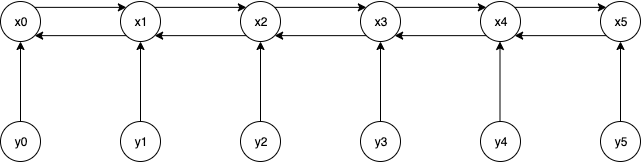
\includegraphics[width=0.8\textwidth]{GraphicalKalmanModel.png}  
  \caption{}
  \label{}
\end{figure}

This graphical interpretation allows us to define an equivalent graph with different dimension nodes 
but the same edges. These are known as $h_x$ and $h_y$ which stands for hidden nodes relating to $x$ 
and $y$ respectively. 

%% Insert another graph here.

The key part of the paper is to define a GNN that operates over this graph with a message passing
routine over the nodes that connect edges and the messages passed in the original 
graph. More specifically for each type of edge, for example $y_t \rightarrow x_t$, we define a 
feedforward neural network that takes the source node, the target node and the message and outputs 
an encoding of the edge, I will refer to these as edge models. These encodings are summed according 
to their source node and then passed through a separate feedforward network which I will call the 
node model. 

The output of this is passed through a GRU along with the previous $h_x$ in order to produce a new 
estimate of $h_x$. The interpretation of this is that edge feedforward networks compute the residual 
error over the edges, the node model computes the residual error left in the $h_x$ and the GRU allows 
some of the past residual error to propagate into the current estimate. The final step passes the new 
$h_x$ through a decoding step to produce an additional corrective factor in addition to $M_t$ called $\epsilon$.

This gives us the final general recursive update rule

\begin{align}
  x_t^{(i+1)} = x_t^{(i)} + \gamma (M_t + \epsilon_t)
\end{align}


\section{My Achievements}

% Some discussion of what I have accomplished. 
% from the booklet "an interesting discussion on what you have achieved in a more global context"

In the HI paper they implement a Kalman Smoother over linear and non linear systems however in both of these cases
they didn't cover the case of having inputs to the system.
%  or using the technique for prediction.

This is necessary in order to be useable in the context of drones as there are inputs required at 
every point, both to maintain stability as well to navigate or accomplish anything useful.

% In order to use the technique in reality both of these capabilities are necessary. For drone 
% control it is clear that there will be inputs to the system, both to keep it stable and also
% to maneuver it to carry out some action. At the same time in order to control a drone effectively
% you need to account for the fact that there will be time lags in some parts of the system. For this
% reason you need to be able to predict a short way into the future for the most effective control.

% Change to the probability function
% \subsubsection{Inputs}

To add inputs I needed to change the probability distribution we are modelling.

\begin{align}
  \hat{\textbf{x}} = \underset{\textbf{x}}{\text{arg max }} p(\textbf{x} | \textbf{y}, \textbf{u}) 
\end{align}
where $\textbf{u}$ are the inputs.

This changes the recursive update function (Eq. 5 in \cite{Satorras2019CombiningGA}) to be 

\begin{align}
  \textbf{x}^{(i+1)} = \textbf{x}^{(i)} + \gamma \nabla_{\textbf{x}^{(i)}}log(p(\textbf{x}^{(i)} | \textbf{y}, \textbf{u}))
\end{align}

% Change to the messages

Which in turn changes the derived input messages to be 

\begin{align}
  \mu_{x_{k-1} \rightarrow x_k}^{(i)} &= \frac{\partial}{\partial x_k^{(i)}} log(p(x_k^{(i)}|x_{k-1}^{(i)}, u_{k})\\
  \mu_{x_{k+1} \rightarrow x_k}^{(i)} &= \frac{\partial}{\partial x_k^{(i)}} log(p(x_{k+1}^{(i)}|x_{k}^{(i)}, u_{k})\\
  \mu_{x_{y_k} \rightarrow x_k}^{(i)} &= \frac{\partial}{\partial x_k^{(i)}} log(p(y_{k}|x_{k}^{(i)})
\end{align}

% Change to the derived matrix operations.

Formulated for the Kalman filter model this gives us

\begin{align}
  \mu_{x_{k-1} \rightarrow x_k}^{(i)} &= -\textbf{Q}^{-1}(x_k - (\textbf{F}x_{k-1} +\textbf{G}u_k))\\
  \mu_{x_{k+1} \rightarrow x_k}^{(i)} &= \textbf{F}^T\textbf{Q}^{-1}(x_{k+1} - (\textbf{x}_k + \textbf{G}u_{k+1}))\\
  \mu_{x_{y_k} \rightarrow x_k}^{(i)} &= \textbf{H}^T\textbf{R}^{-1}(y_k - \textbf{H}x_k)
\end{align}

Where $\textbf{G}$ is the gain matrix over the inputs $u$.

In a wider context this is a small but significant extension that shows that this technique
could be used in the full spectrum of applications of the Kalman Smoother. 

I detail the implementation in Work Completed and share the results which are comparable 
with the original HI implementation.

% Extension to prediction.

% \subsubsection{Prediction}

% In order to extend to prediction 


%%%%%%%%%%%%%%%%%%%%%%
%%% Work Completed
\chapter{Work Completed}

%%% Written Summary
\section{ROS and Gazebo}

%% install ROS and Gazebo
The first task to carry out was to install ROS and Gazebo. As mentioned earlier ROS is the framework 
into which my code will fit. Gazebo is a simulation tool that I will be using to verify everything 
before deploying anything in reality. Luckily Gazebo is included with ROS (with some exceptions) so 
installing it separately is not necessary. If you need the most recent version of Gazebo this is not 
true, you need to follow some additional steps to install it and link it with ROS so they interact 
correctly.

I did have some confusion about which version of ROS I needed to be compatible with various things 
but I made the decision to stick with the most recent version of ROS and the standard version of 
Gazebo packaged with that. This simplifies the setup for anyone seeking to reproduce my project.

The ROS website\cite{melodic/installation/ubuntu} has an excellent guide on installing ROS for the 
first time on Ubuntu and I highly recommend it.

%% install hector code

%% explain catkin workspace.

After that I installed the hector stack. This was quite a long process of trial and error as there 
does not seem to be a guide for getting started with this set of packages. I first tried to install 
them from apt as they are available there. That did not work and I believe the issue is that they 
were built for an earlier version of ROS but packaged for melodic without any changes. Regardless 
of the reason that did not work. I was trying to install the hector quadrotor and hector gazebo 
packages as those were the only packages that I believed that I needed. I tried to clone them into 
the src folder of my catkin workspace. While trying to build it failed because of dependencies on 
other hector packages, namely hector slam hector models and hector localization. Then it was missing 
the geographic mesages. Then it failed because it was missing qt4. I installed both of those with 
apt. The full process took a while longer than this explanation as you only find out anpther 
dependency is missing after building again. A final issue was that the memory usage at certain 
points spikes. It turned out that this was causing the VM to run out of memory and stop compliation. 
This caused very confusing error messages as they didnt seem to be for anything in particular. I 
finally figured out with the help of htop and allocated more memory to the VM which solved the issue. 
One anachonism of this stack is that it doesn't seem to build in the right order. It will often fail 
only to complete more after rerunning. At one point it was necessary to continually rerun catkin\_make 
about 7 or 8 times in a row. The only cause for concern is when it stops at the same percentage built more 
than once. 


\section{Hardware for Demonstration}

%% evaluation of alternatives
My original plan was to use a Raspberry Pi for onboard computation when I transition to 
operating on the physical drone rather than in Gazebo. This was for a couple of reasons, primary was 
the low power draw while still offering gigahertz computation. I have a Raspberry Pi 2 and I planned 
to purchase a Raspberry Pi 4 for the final implementation due to its increased compute power.

%% selection of Jetson Nano
While experimenting with my RasPi 2 I found some limitations with its implementation of Python as 
well as concerns about its prospective performance due to reports found online. I researched 
alternatives, as there are a wide variety of Single Board Computers on the market now. While looking 
I found that NVIDIA produce the Jetson Nano and specifically the SDK kit, which is very similar to 
the RasPi but has native support for PyTorch, the deep learning library I am using as well as having 
128 GPU cores. This enables me to take advantage of parallelised matrix computation with the 
associated performance improvements. On top of this it only consumes up to 10W of power, admittedly 
this is double the 5W draw of the RasPi but 10 is the maximum, not necessarily what it will consume. 
I will explore power consumption in the second part of the project.

%% installation of PyTorch and ROS.
After the Nano arrived I installed PyTorch and ROS onto it. This allowed me to verify the steps 
needed for installing both packages and ensure the most streamlined set of instructions.

There were some issues with the original version of PyTorch installed due to the Nano using
an ARM CPU. This means that it has the aarch64 architecture and so compiled executables are trickier
to get hold of and often are not quite the same as x86. In this case PyTorch uses some external 
libraries for some of the matrix operations, these include OpenBLAS and MKL. In the first version 
I installed these were not present, preventing matrix inverse operations. This is critical 
to both Graphical Kalman Smoother and by extension the HI implementation.

I tried a number of solutions including installing from source however in the mean time an updated
version of PyTorch was released for the Nano which included OpenBLAS solving the problem.

In the end there were a number of factors that prevented the eventual hardware integration.

% I will still try and profile the time and power requirements of running the code for SLAM.


\section{TUM code}

%% Go through the process. Look at the diary.
The first step in working with the TUM code was to compile it. I was aware that it was written to 
target ROS Fuerte with some modifications to support Indigo which is 3 versions behind Melodic.

I first attempted to build the project on the Jetson Nano as I was planning to use it as my 
development platform as well as the deployment environment if possible. This was not possible. The 
build failed due to a dependancy, ardrone\_autonomy. This is a wrapper for the Parrot AR drones SDK. 
It also provides a number of message definitions. I attemped first to build the dependancy on the 
Nano but there are issues with compiling that code on an ARM platform. This prompted me to drop the 
dependancy and the speed of compilation prompted me to abandon the Nano for development.

I found that the only code from the ardrone\_autonomy package were the messages. I then extracted 
the message definitions from the ardrone\_autonomy package into my own package.

After solving that issue I ran into much more serious issues with a third party library called 
libcvd which is an OpenCV alternative that PTAM, the monocular SLAM component.
This package is packaged as a thirdparty library inside a tarball with two other libraries.
Upon building it would fail on apparently legal C++ code. I tried to use the most recent version of 
libcvd, pulling it from github, building and installing it on the system separately. This didn't work 
so I tried placing it into the thirdparty tarball. That also did not work. I found that the directory
structure of the new version did not match the original and there was a Makefile I needed to 
replicate. I then found that there were some files that had been deprecated but the TUM code relied 
upon so I pulled them over from an old version of the library. This on it's own did not fix the 
issue but when I found a final Makefile I could add the files I had pulled over into the list of 
artifacts that would be made available by that stage of the build. 

Then I found some namespace issues as another dependency was not being found in the expected manner.
I had to set a definition in order to fix that problem. I also had to remove the GUI section of the 
code as it had more serious persistent issues. If I have time spare after completing the project I 
will go back and try and fix that as well. Finally there was a section of code that relied upon 'tf', 
which is a geometry package of ROS but is now deprecated. I had to rewrite that section to use 'tf2' 
which is the replacement for 'tf'.

After building it ran without issue.

I then explored how to get it to interact with the hector stack. I looked through the hector stack and it is 
very large. A lot of it is not needed for my project so I considered extracting the core functionality
that I want, create a world with a quadcopter that acts correctly. Unfortunately the hector stack 
has a large number of interdependencies so it is infeasible to extract only certain components, at 
least not at this stage. I have identified where they will interface. They use different conventions 
for positions so I need to create an adapter.

\section{Hybrid Inference}

%% Create the dataset
\subsection{Data}
% understand the linear models, create one (discrete vs non discrete)
A prerequisite for any task that includes neural network is collecting or creating the data for it 
to train on. In this case my dataset is created as at this stage I am firstly verifying that the 
technique works as expected and I can implement it. After this stage I will formulate the real 
problem and collect data in Gazebo for that stage.

My dataset consists of position data generated by a simple linear model with Gaussian noise in the 
transition matrix as well as the measurement matrix. This is very similar to one of the experiments 
carried out in \cite{Satorras2019CombiningGA}. This is intentional in order to have comparison data,
though the model I am using is likely to be much simpler than that used in the paper.

% testing
The testing strategy I have used for the Linear Model and the Dataset is designed to verify the core
performance. That the amount of data created is correct, that the various options operate as expected 
and that the output data is in the format expected.

%% Create the Kalman filter
% understand and formulate
\subsection{Graphical Model, GNN and Hybrid Inference}

My original understanding of the Hybrid Inference formulation was that the graphical model was a 
regular Kalman Filter and the GNN was formulated in a similar fashion. As I describe in the Background 
Theory section that is not the case. The graphical model is a reformulation of the problem and 
solution. I realised this after reading the paper with reference to the GitHub repository with their 
implementation \cite{vgsatorrasgithub}. It took a fairly long time to understand their code as it is 
not really documented and has a somewhat confusing structure.

Implementing the graphical model was then relatively straightforward though trying to keep it self 
contained and modular complicated things slightly. My implementation of the GNN is quite problem 
specific. At the moment I can't see much way to make it more generic. Given that I will have to 
reformulate for the reasons just stated I will explore where the commonalities are and whether a 
generic version is feasible or desireable. It differs quite a lot from the Satorras' formulation 
mainly due to my desire to improve the interpretability of the code and give a cleaner flow and 
structure. Functionally they are equivalent except that my node model is a 3 layer feedforward 
network whereas the one they implement is 2 layers. I also decided not to implement different 
modes for graphical only or GNN only as I specified these as separate standalone, or semi 
standalone in the case of the GNN, classes. As I had implemented the two components separately 
it made the Hybrid Inference class very simple as it is just a composition of the two.

% The current implementation really implements a Kalman Smoother, that is an optimal estimate of past 
% observations, not a real time filter or predictor which is really what is needed for the full 
% realisation of this project. The key challenge in extending it to the realm of prediction is the fact 
% that some of the messages will become meaningless, particularly the $y$s or observations that we 
% have not observed yet. It is possible that using zeros is a possible solution though it is not 
% certain.

% Another challenge that came up in this section of work is the fact that the Hidden Markov process 
% that I am modelling is slightly different to the one evaluated by Satorras et al.

% The state transition they evaluate is 
% \begin{align}
%   x_t &= Ax_{t-1} + Q_t
% \end{align}

% But the state transition for a drone will actually be
% \begin{align}
%   x_t &= Ax_{t-1} + Gu_t + Q_t
% \end{align} 

% Where $G$ is the input gain matrix and $u_t$ is the input at time $t$.
% This is not a problem but it will require me reformulating the graphical model and the respective 
% messages. This is not something that I had anticipated so this will figure into my plans for next 
% term.

In the second term I focused initially on the HI section of the project. I first sought to 
verify the results of the HI paper before continuing with solutions to the challenges identified 
at the end of the first term. Namely that of inputs and that of prediction.

Firstly I compared the HI model with the graphical formulation of the Kalman Smoother.
Initially the results were significantly worse which is not supposed to ever happen.
This triggered an in depth review of my implementation to find the source of the error.
Every line was stepped through and evaluated, my initial idea was that the GNN part 
of the implementation was the most likely culprit. I finally discovered that the cause 
was the number of iterations that the HI implementation carries out before returning the 
solution. It was 50 compared with the Graphical Kalman Smoother using 200. Once they were
equalised the HI performed better.

% That resolved I tackled the prediction problem.

% Then implementing it for the drone case.

% Then gathering data from Gazebo.

% Then integrating it into hector.

%%%%%%%%%%%%%%%%%%%%%%%%%%%
%%% Work completed in the second term..

% \section{Second Term}

% %%% Hybrid Inference
% % work out the formulation and implement for the case of the quadcopter
% The first thing to be done is to solve the two problems identified during this terms work on HI.
% First is that HI as described 
% in the paper, deals with a simplified linear dynamic model that does not have inputs to the system.
% The dynamic model that describes MAVs must include external inputs for control. Reformulating the 
% graphical model to account for this is the first new challenge that I had not identifiend in the 
% initial project plan. The second challenge is temporal. With a Kalman Filter, it is possible to 
% estimate future states and the uncertainty of those postulated states. This is critical for dealing 
% with latency issues in the real time control environment that MAVs present. The current formulation 
% of the underlying graphical model does not allow for future reasoning, solving this is necessary to
% enable HI to be used this domain. Once that is done I can implement the new formulation and train it 
% on data gathered from Gazebo.

% %%% ROS and Gazebo
% On the ROS and Gazebo side, I will simulated a drone in order to capture data to train the HI 
% implementation and I will write a node that carries out the HI and returns 
% pose estimates to the control module. This will allow me to fully demonstrate the technique and 
% its effectiveness.

% %%% Hardware
% Time permitting I will at this point be focusing on real life demonstration. For that I will 
% integrate the Jetson Nano with the Matrice 100. This requires a voltage adapter to power the 
% Jetson from the Matrice and a USB to UART connector. These a both commercially available. 
% After that I will have to establish communication and integrate the ROS code that I have developed 
% with the DJI OSDK. I will write an adapter node that deals with the DJI OSDK and accepts commands 
% from the cmd\_vel Topic which is the canonical way to issue control commands. This will allow the 
% code I write to be drone agnostic with an adapter being all that is needed to use my code on any 
% other drone. To demonstrate the technique I will have the drone perform precision figures in a 
% similar fashion to \cite{Engel:FigureFlying}.

% Finally, with available time I will profile the technique against the Extended Kalman Filter and
% attempt to quantify the computational resources required for its operation.

% The tasks and timing are best represented in the Gantt Chart below
% \begin{figure}[h]
%   \centering
%   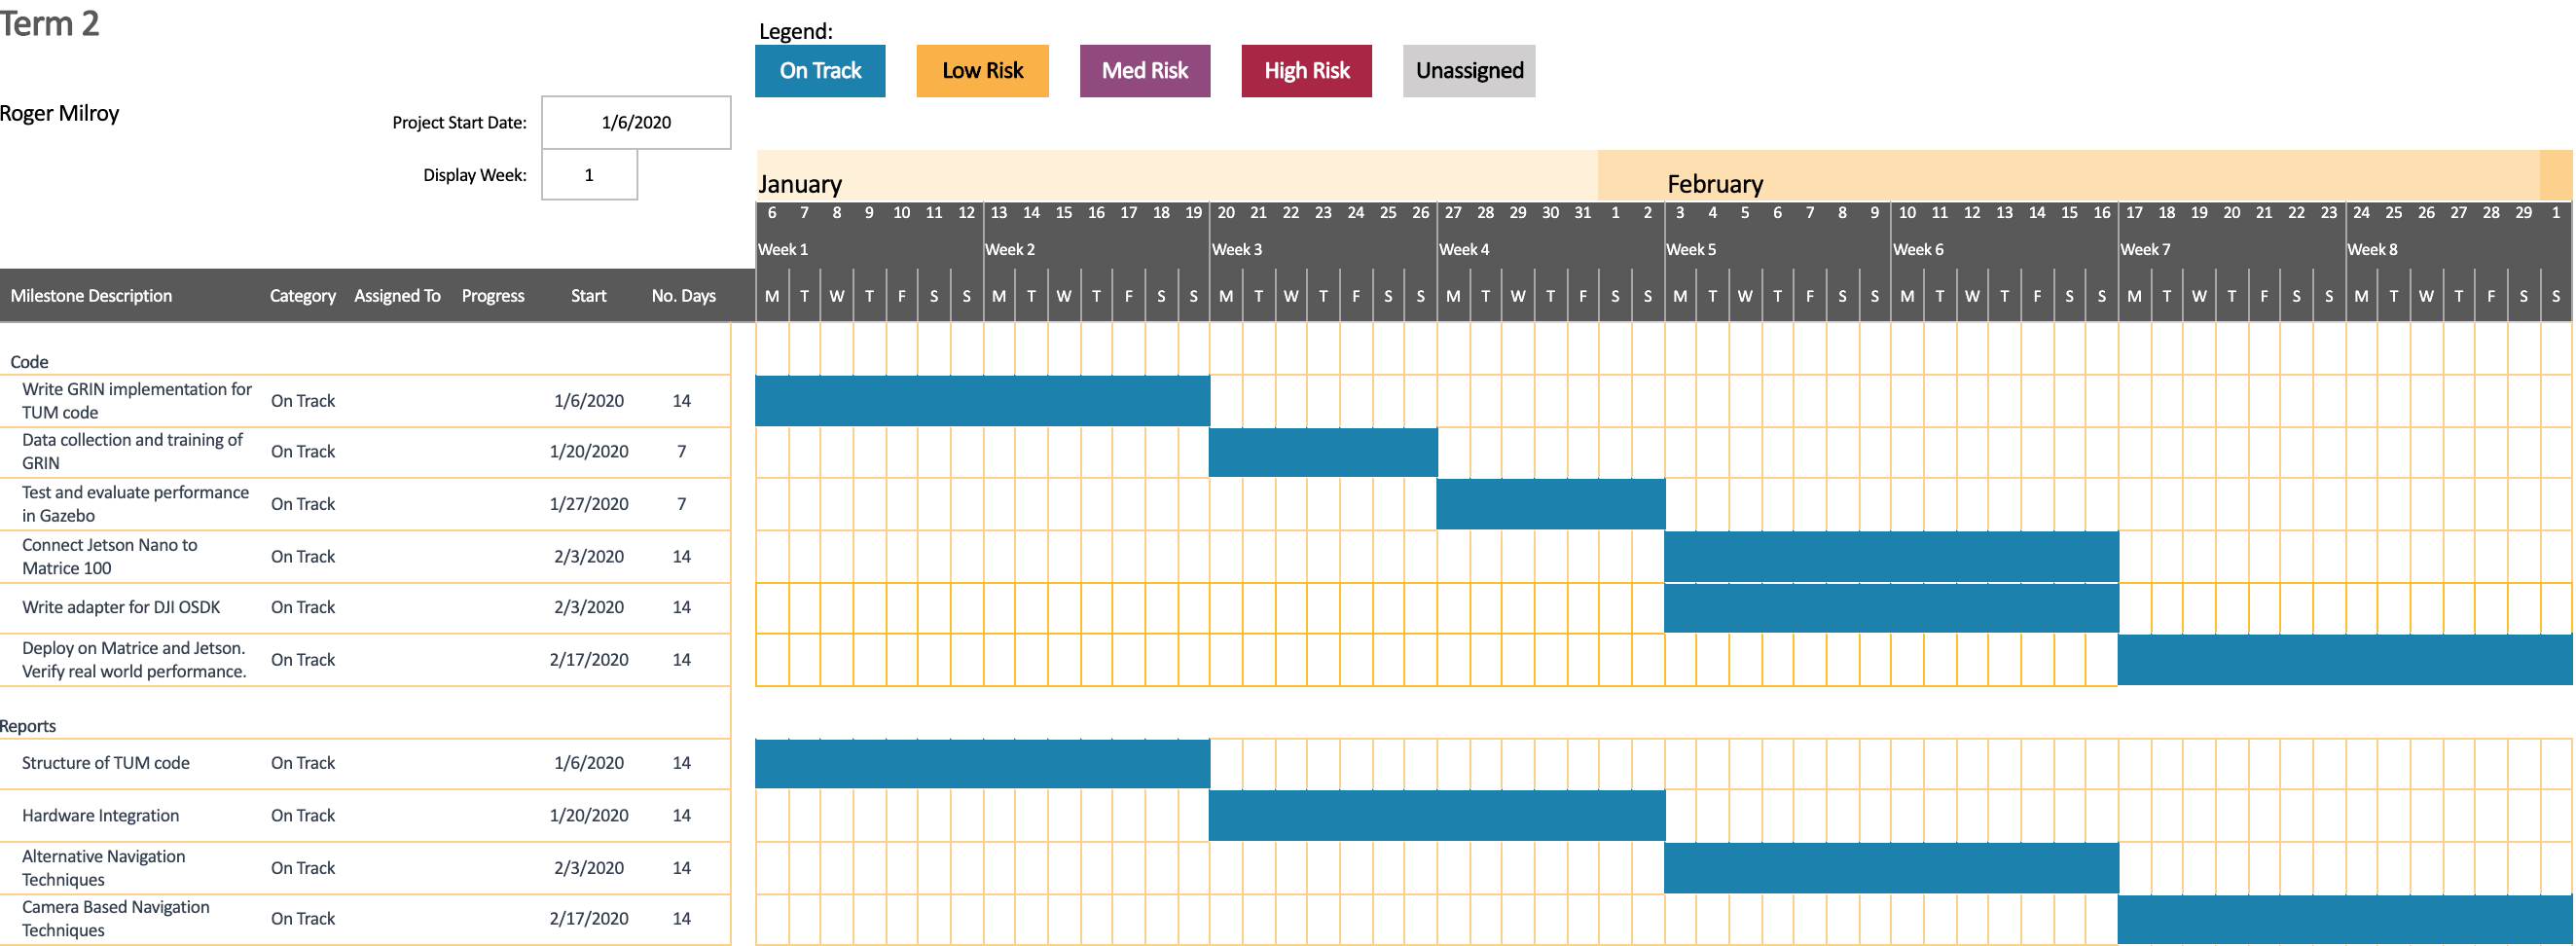
\includegraphics[width=\textwidth]{Term2GanttChart.png}  
%   \caption{Term 2 Gantt Chart.}
%   \label{}
% \end{figure}


%%%%%%%%%%%%%%%%%
%%%% Self Evaluation

\section{Self Evaluation}

% How did the project go?
I would consider the project to have gone reasonably well. I certainly had plenty of 
challenges and some scaling back of ambition but I am happy with the final results that 
I was able to achieve.


% Where next? 
The next stage of this project will be to actually integrate it with some hardware.
Due to the complications encountered I had to scale back my ambition to remain at the
simulation level.


% What did you do right/wrong? 
In terms of process, I would say that my consistency of work was good, I managed my time
pretty well in relation to other commitments balanced with this one to ensure that there 
was some measure of progress each week.
In terms of individual decisions, I think that the decision to focus on the Hybrid Inference 
technique was a good one in terms of enabling me to challenge myself, learn a large amount 
about new areas of theory, notably in Hidden Markov Models, Kalman Filters and Graph Neural Networks.

I would say that I did a few things wrong. The first was not doing enough research before the
project started. I should have spent more time checking for all the resources I could use. 
A key example of this was the Monocular SLAM project I wanted to replicate. I found that it was 
open source and more generic than I had assumed so I could reuse it. This led to me pivoting
my project aims to focus more on Hybrid Inference.
Following on from that, I was far too ambitious in my original planning. I had planned to 
implement two serious papers techniques, integrate them in Gazebo and then also on the DJI
Matrice. This was far too optimistic as was evidenced by the change in project aims and
scaling back of ambition.


% What have you learnt about doing a project?
The key takeaway for me is the limitations of the Waterfall method of project planning and 
management.
This project was structured as some version of Waterfall in that we planned the deliverables,
milestones, timing and essentially every part of the project right at the start of the project.

This has some advantages in that it forces you to spend some time thinking about the project which
should reduce the amount of surprises. The downside is that many things change during the course of
a project of this size and duration. Particularly for those of us working with entirely new 
technologies in different application areas than we have worked on before, ie. not some kind of web
app or desktop/mobile application, it is very hard to estimate the amount of time needed for
most of the tasks we were planning. Unsurprisingly many ended up taking much longer than estimated.

I think that preplanning is necessary but the extent and detail must vary depending on the extent 
of familiarity with the domain, tools and task to be carried out. In any case there will often be 
regular course checks and this is where the Agile approach has significant advantages in setting
short term goals that are better understood and more controllable over large goals over
longer time periods where the scope for misunderstanding is much greater.

The other thing that I have learned about doing a project is that fixing issues generally 
takes much more time than implementing new functionality. At the same time it is much 
harder to plan your time when fixing issues as there is no reasonable way to estimate when
you will understand the issue enough to solve it. This is much more of a problem when using
little used tools or technologies. For the majority of application development there is 
a large amount of knowledge available online to refer to when encountering difficulties. 
Unfortunately for me ROS and Gazebo have more limited communities using them. And when 
implementing new techniques, there is no reference other than the paper, and maybe source code
if made available via GitHub.


%%%%%%%%%%%%%%%%%
%%%% BIBLIOGRAPHY

\newpage
\bibliographystyle{acm}
\bibliography{../resources/final_project}
\nocite{*}

\label{endpage}

\begin{appendices}

  
\end{appendices}
  
\end{document}

\end{article}